\documentclass[parskip=half]{scrartcl}

\usepackage[english]{babel}
\usepackage[perpage]{footmisc}
\usepackage{csquotes}
\usepackage{hyperref}
\usepackage[backend=biber, sorting=none, style=nature, date=year, urldate=ymd, isbn=false, url=false, doi=true, eprint=false]{biblatex}
\usepackage[top=2cm, bottom=3cm, left=2cm, right=2cm]{geometry}
\usepackage{amsmath}
\usepackage{amssymb}
\usepackage{booktabs}
\usepackage{cleveref}
\usepackage{algorithm}
\usepackage{algpseudocode}
\usepackage{braket}
\usepackage{xcolor}
\usepackage{expl3}
\usepackage{xparse}
\usepackage{tcolorbox}
\usepackage{tikz}


\addbibresource{sources.bib}


% https://tex.stackexchange.com/a/152310
\deffootnote[0em]{1em}{0em}{\textsuperscript{\thefootnotemark}}

% use roman footnote numbers
\renewcommand{\thefootnote}{\Roman{footnote}}


%%%%%%%%%%%%%%%%%%%%%%%%%%%%%%%%%%%%%%%%%%%%%%%%%%%%%%%%%%%%%
%%%%%%%%%%%% DEFINITION OF CUSTOM MACROS %%%%%%%%%%%%%%%%%%%%
%%%%%%%%%%%%%%%%%%%%%%%%%%%%%%%%%%%%%%%%%%%%%%%%%%%%%%%%%%%%%

\ExplSyntaxOn

% Macro for typesetting a permutation in cycle notation
\NewDocumentCommand{\perm}{ m }{
	\seq_set_from_clist:Nn \l_tmpa_seq { #1 }
	(\seq_use:Nnnn \l_tmpa_seq {\;}{\;}{\;})
}
% Macro for typesetting a permutation's image with superset element indices
\NewDocumentCommand{\image}{ O{} m }{
	\ensuremath {
		\seq_set_from_clist:Nn \l_tmpa_seq { #2 }

		[\,
			\seq_indexed_map_inline:Nn \l_tmpa_seq {
				\int_compare:nF { ##1 = 1 } { , }
				\overset{{\color{gray}\scriptscriptstyle\int_eval:n { ##1 - 1 }} } { \mathstrut #1{##2} }
			}
		\,]
	}
}
% Macro for typesetting a sequence of elements, with superset element indices
\NewDocumentCommand{\sequence}{ m }{
	\image[\textrm]{#1}
}


\cs_new:Nn \if_math_mode:TF {
	\relax\ifmmode
		#1
	\else
		#2
	\fi
}

\NewDocumentCommand{\code}{ m }{ \texttt{#1} }
\NewDocumentCommand{\class}{ m }{ \code{#1} }
\NewDocumentCommand{\libPerm}{ }{ \texttt{libPerm} }
\NewDocumentCommand{\Sym}{ m }{
	\if_math_mode:TF{
		\textrm{Sym}(#1)
	}{
		Sym($#1$)
	}
}
\NewDocumentCommand{\complexity}{ m }{
	\ensuremath{
		\mathcal{O}(#1)
	}
}

\ExplSyntaxOff



\author{Robert Adam}
\date{last edited: \today}
\title{\libPerm}


\begin{document}
	\maketitle

	\tableofcontents

	\cleardoublepage


	\section{Motivation}

	In another project, we needed to deal with the permutational symmetries of indices of tensor elements that take the form of e.g.
	\begin{equation}
		T^{ab}_{cd} = - T^{ab}_{dc} = -T^{ba}_{cd} = T^{ba}_{dc}
	\end{equation}
	In order to be able to perform any kind of automatic simplifications on expressions involving tensor elements with such symmetries, it is clear
	that a way to determine if two tensor elements are equivalent (in the sense that they can be written in the form $A = \pm B$) is necessary.

	The best approach for dealing with symmetry-related questions like that, is to turn to group theory. Therefore, we needed a library to properly
	deal with permutation groups. Since the main project was in C++, so should that library. A search on the web produced \textcite{PermLib} that
	seemed to fit the purpose perfectly. Unfortunately, this library has become quite outdated and does not even compile on somewhat modern
	systems. However, its author has written his thesis about the implementation\supercite{Rehn2010} and in there were suggestions for how to treat
	permutation groups efficiently. Thus, we went ahead and created our own implementation.


	\section{Notation}

	\Cref{tab:notation} summarizes the symbols and concepts used throughout this work (unless noted otherwise). We assume the reader is generally
	familiar with group theory basics and thus will not include a full introduction here.

	Furthermore, note that we start enumerations at zero rather than at one (unless noted otherwise).

	\begin{table}[!h]
		\centering
		\caption{Common notation and concepts used throughout this document}
		\label{tab:notation}

		\begin{tabular}{p{.12\textwidth} p{.63\textwidth} p{.15\textwidth}}
			\toprule
			\textbf{Notation} & \textbf{Concept} & \textbf{Def. / Ref.} \\
			\midrule
			\Sym{n} & Symmetric group of $n$ elements & \textcite{Wiki_SymmetricGroup} \\
			$P, G, H$ & General (permutation) group & \\
			$p, g, h$ & An element of the respective group & \\
			$\alpha, \beta, \ldots$ & Concrete integer number ($\alpha, \beta, \ldots \in \mathbb{Z}_0$) & \\
			$\alpha^g$ & The image of $\alpha$ under the action of $g$ & \\
			$|G|$ & The order (amount of elements contained) of the group $G$ & \\
			$gh = g \cdot h$ & Product of $g$ and $h$. Please see \cref{sec:CompositionOrder} for what exactly this means. & \\
			$gH$ & The left coset of $g$ with $H$. Note that (usually) $g \in G$ and $H \subseteq G$ & $\{ g h | \forall h \in H \}$ \\
			$Hg$ & The right coset of $g$ with $H$. & $\{ h g | \forall h \in H \}$ \\
			$id$ & The identity permutation & \\
			\bottomrule
		\end{tabular}
	\end{table}


	\section{Applying permutations and order of composition}
	\label{sec:CompositionOrder}

	When we \enquote{multiply} two permutations $a$ and $b$, we create a new permutation $c = a \cdot b$. This new permutation is then the
	\emph{composition} of its \enquote{factors}. Composing two permutations effectively means first applying one of them and then applying the other.
	The only question remaining is this: given $c = a \cdot b$, do we first apply $a$ or do we first apply $b$?

	Someone coming from maths will immediately think of function composition $h = g \circ f$, where the composition is understood to mean
	$h(x) = g(f(x))$. That is, the order of applying the functions is from right to left. However, when dealing with permutations, it is common to
	instead use a left-to-right interpretation of composing two permutations, such that $a \cdot b$ is understood as first applying $a$ and then
	applying $b$. Thus, composing permutations works left-to-right.

	However, this is only valid as long as the permutations are only applied to a single integer. This, by definition, gives the image of that number
	under the acting permutation $\alpha^a$. There is also the possibility to let a permutation act on an entire sequence of elements, in which case
	the elements in the sequence shall be rearranged according to the permutation. Since the elements in that sequence don't have to be integers, it
	is clear that the permutation must somehow act on the indices of the elements instead of the elements itself. But still, there are two possible
	ways to do that:
	\begin{enumerate}
		\item The $\alpha$-th element in the original sequence will be moved to position $\alpha^a$ in the rearranged sequence
		\item The $\alpha$-th element in the rearranged sequence will be the $\alpha^a$-th element of the original sequence
	\end{enumerate}

	We choose to use the second interpretation as this is the one in which a sequence of integers \image{0, 1, 2, \ldots} will be mapped to
	\image{0^a, 1^a, 2^a, \ldots} when acting on it with the permutation $a$.

	If we call our sequence $s$ and denote the $\alpha$-th element of the sequence as $s[\alpha]$, we can formalize what it means for a permutation
	$p$ to act on $s$:
	\begin{equation}
		s^p[\alpha] = s[\alpha^p]
	\end{equation}

	If we instead apply two permutations to the sequence one after the other, say first $a$ and then $b$, the situation would look as follows:
	\begin{equation}
		s^{ab}[\alpha] = \left( s^a \right)^b[\alpha] = s^a[\alpha^b] \overset{\beta=\alpha^b}{=} s^a[\beta] = s[\beta^a]
		= s[(\alpha^b)^a] = s[\alpha^{ba}]
	\end{equation}

	Therefore, it can be seen that the meaning of the composite permutation $ab$ is exactly reversed when acting on a single integer ($\alpha$) vs.
	when acting on a sequence ($s$). Since permutations are by definition defined as a bijection of a set of numbers onto itself, the composition
	order of applying a permutation to an integer, is the \enquote{natural} composition order that we chose. Therefore, while composition of
	permutations acting on integers are ordered left-to-right, permutations acting on sequences act right-to-left.

	An example where this comes into play is if you have two permutations $a$ and $b$ and apply them to your object individually, first $a$ and then
	$b$, and then want to construct a composite permutation $c$ that performs these two steps in a single action. If your object is an integer, then
	$c = ab$, but if your object is a sequence that you want to permute, $c = ba$.

	\begin{tcolorbox}[colback=red!5!white,colframe=red!75!black,title=Composition order]
		\begin{itemize}
			\item When acting on integers, permutations compose left-to-right
			\item When acting on sequences, permutations compose right-to-left
		\end{itemize}
	\end{tcolorbox}


	\section{Usage}

	Might come eventually. For now, see the examples directory in the source repository.


	\section{Implementation}

	The focus of our implementation is to arrive at a fast and efficient library primarily aimed at dealing with small permutation groups $P \subseteq
	\Sym{n}, n \sim 10$. In order to do this, the library tries to avoid dynamic memory allocations wherever feasible (another big difference to
	\textcite{PermLib}). The library is implemented according to the ISO C++17 standard.

	C++ comes with the restriction that when working with objects through their base-class interface, it is (without tricks) impossible to e.g. create
	a copy of the object without resorting to dynamic memory allocations\footnote{The reason for this is that the compiler needs to know the exact
	size of a given object, if it is to be created on the stack and in terms of polymorphic types, the size of the actual underlying object is only
	determined at runtime.}. However, by assuming that we will never have to deal with implementations of our interfaces from outside our library, we
	can assume that we know all possible implementing classes of a given interface at compile-time. This special case of polymorphism is called
	\emph{closed-set} polymorphism and it allows us to use a trick leveraging the \class{std::variant} class in the standard library. The details of
	this are not important here, but the effect is that this allows us to treat polymorphic objects as \emph{value-types}\footnote{Types that can be
	moved around, copied and stored (in containers)}. For this purpose, we have implemented another library
	\code{polymorphic\textunderscore{}variant}\supercite{polymorphic_variant} that encapsulates all the unmentioned details of this trick.

	In the following, if we refer to an interface being \emph{unwrapped} into a new type, that corresponds to creating a
	\code{polymorphic\textunderscore{}variant} wrapper for the closed-set polymorphism for the given interface (aka: collect all existing
	implementations of that interface into a single wrapper type).

	The only thing to be aware of, is that you'll have to use the arrow operator (\code{->}) to access member functions for unwrapped types. E.g.
	\code{perm->isIdentity()} instead of \code{perm.isIdentity()}.


	\subsection{Representing permutations}

	The most fundamental object that a library dealing with permutation groups has to have, is a way to represent a single permutation. There are
	multiple possible ways of achieving this task, each having their distinct advantages and disadvantages. 

	Since this is a C++ library, permutations are represented as the bijection of a set $S$ onto itself, where the points in $S$ start at zero,
	rather than at one (as is common practice when working with permutations in e.g. a maths context).


	\subsubsection{\texorpdfstring{\class{AbstractPermutation}}{AbstractPermutation}}

	In order to be able to be able to test or switch out the used representation in \libPerm, we created the \class{AbstractPermutation} interface.
	This interface covers all functionality that the library or any user of the library is expected to require in order to work with a given
	permutation. This covers basic operations like comparing for (in)equality, computing the image of a point under the represented permutation,
	checking for identity, inverting the permutation in-place and of course to multiply two permutations.

	One consequence of choosing runtime polymorphism in order to allow for multiple implementations of permutation representations is that the general
	interface can't include any operation that itself returns a permutation object. The reason for this is that such an object would either have to be
	allocated dynamically (which we want to avoid) or the function signature in the interface would have to enforce one specific implementation as the
	return value (instead of returning the by interface)\footnote{The underlying reason for this is again that the compiler can't deduce the actual
	size of the respective object}. As a result, the general interface does not include a binary multiplication operator, that takes two permutations
	and creates a new one. Instead, only the multiply-assign (in-place multiplication) operator is provided, that multiplies two permutations \code{A}
	and \code{B} and then sets \code{A} to the result of the multiplication (thereby avoiding the need to create a new permutation object).

	In contrast to the classical definition of permutations, the \class{AbstractPermutation} interface also allows permutations to carry a sign
	information. This property is completely orthogonal to the underlying permutation itself. However, it is transformed accordingly when e.g.
	multiplying or inverting permutation objects. The reason for adding this additional property is that dealing with signed permutations is required
	in the context of tensor symmetries and it is a lot easier to just integrate that into the main interface than injecting this property by other
	means.


	\subsubsection{\texorpdfstring{\class{Permutation}}{Permutation}}

	The \class{Permutation} \enquote{class} is simply the result of \emph{unwrapping} the \class{AbstractPermutation} interface.


	\subsubsection{\texorpdfstring{\class{ExplicitPermutation}}{ExplicitPermutation}}

	The \class{ExplicitPermutation} class is a concrete implementation of the \class{AbstractPermutation} interface. It stores a permutation as a list
	of points, where the $i$th point corresponds to the image of $i$ under the represented permutation (\code{list[$\alpha$] = $\alpha^{g}$}, where
	$g$ is the represented permutation). Note that this class will always explicitly store the images of the set $\{ 0, \ldots, n \}$, where $n$
	is the biggest element affected by the represented permutation. Always explicitly representing the images of (potentially unchanged) lower points
	avoids excessive branching in the remaining implementation.

	The idea for using this representation is taken from \textcite{Rehn2010} (they called this form \enquote{elementary permutations}). As noted
	there, this representation has the advantage of providing access to the image of a point $\alpha$ under the represented permutation $g$ in
	\complexity{1}. Multiplying an \class{ExplicitPermutation} with another (arbitrary) \class{Permutation} can be performed by
	\cref{alg:MultiplyExplicitPermutation}. If we assume that looking up the image of a point under the \class{Permutation} is \complexity{1} (which
	is the case, if e.g. multiplying two \class{ExplicitPermutation} with one another), then this multiply operation can be performed in
	\complexity{n}\footnote{This is in contrast to what is stated in \textcite{Rehn2010} who state that such multiplication can only be performed in
	\complexity{n^2}.}.

	\begin{algorithm}
		\caption{Algorithm for multiplying an \class{ExplicitPermutation} with an arbitrary \class{Permutation}. Complications arising from the second
		permutation acting on a larger set of points that the first one are left out for brevity.}
		\label{alg:MultiplyExplicitPermutation}
		\begin{algorithmic}[1]
			\Function{multiply}{\class{ExplicitPermutation} $a$, \class{Permutation} $b$}
				\ForAll{image points $\alpha$ in $a$}
					\State $\alpha \gets \alpha^b$
				\EndFor
			\EndFunction
		\end{algorithmic}
	\end{algorithm}

	Inverting an \class{ExplicitPermutation} can be performed by \cref{alg:InvertExplicitPermutation}, which also scales as \complexity{n}.

	\begin{algorithm}
		\caption{Algorithm for inverting an \class{ExplicitPermutation}.}
		\label{alg:InvertExplicitPermutation}
		\begin{algorithmic}[1]
			\Function{invert}{\class{ExplicitPermutation} $p$}
				\State \code{inverted}: List for the inverted image points
				\For{$\alpha \in [0, $ length of \code{inverted}$) \wedge \alpha \in \mathbb{N}_0$}
				\State $\code{inverted}[\alpha^p] \gets \alpha$
				\EndFor
				\State Use \code{inverted} as new image points
			\EndFunction
		\end{algorithmic}
	\end{algorithm}

	One big advantage of using a direct storage of the image points over e.g. \enquote{permutation words}\supercite{Rehn2010} is that operating on the
	former can be expected to be cache-friendlier due to the avoidance of a linked-list-like structure\footnote{At least for permutations acting on a
	reasonably small (probably $<100$) set of points.}.


	\subsection{Representing permutation groups}

	A permutation \emph{group} is just a collection of individual permutations, that together form a \emph{group} (in the mathematical sense). The
	most trivial way of representing a permutation group is therefore to just represent it as a list of \class{Permutation} objects. However, this
	incurs some disadvantages when working with the group. One disadvantage is that the order of a permutation group increases very rapidly (the order
	of \Sym{n} is $n!$) and therefore, explicit storage can quickly become costly and eventually impossible. Therefore, permutation groups are often
	represented in a compressed way by means of a \emph{base} and a \emph{strong generating set} (together: BSGS) as obtained by the so-called
	\emph{Schreier-Sims algorithm} (for details see e.g. refs.~\cite{Butler1991a, Rehn2010}).


	\subsubsection{\texorpdfstring{\class{AbstractPermutationGroup}}{AbstractPermutationGroup}}

	Similarly to the \class{AbstractPermutation} interface, we also created a general interface for a general permutation group, which we called
	\class{AbstractPermutationGroup}. The interface tries to cover common operations one would like to perform on a permutation group, such as
	computing the \emph{orbit} of a point $\alpha$ under the group $P$. Other supported operations include getting the group's order, performing
	membership tests\footnote{Answering the question \enquote{Does this group contain permutation $p$?}}, adding a (new) generator for the group,
	recomputing the group from a given set of generators, explicitly obtaining a list of all elements of the group and getting the \emph{canonical
	coset representative} (see below).

	\paragraph{Canonical coset representative} Any element contained in a coset, can be chosen as a \emph{coset representative}. However, it is
	beneficial if the act of choosing such a representative is defined in such a way that, given a coset, the chosen representative will always be
	the same (regardless of e.g. the order in which the coset's elements are in). If this is fulfilled, the chosen representative will be called a
	\emph{canonical} coset representative.


	\subsubsection{\texorpdfstring{\class{PrimitivePermutationGroup}}{PrimitivePermutationGroup}}

	The \class{PrimitivePermutationGroup} is an implementation of the \class{AbstractPermutationGroup} interface, that essentially follows the trivial
	approach outlined before: it stores the elements of the group explicitly in a list. Additionally, the group maintains a separate list of
	generators. The latter turned out to be beneficial when e.g. trying to extend a group with a new generator.

	The group is intended to be constructed from a set of permutations that \emph{generate} the group. Since we want to represent the group by
	explicitly storing all of its elements, one fundamental task in this implementation deals with generating these elements from a set of generators.
	The most efficient way (known so-far) to accomplish this to use \emph{Dimino's algorithm}.\supercite{Butler1991a} A detailed \enquote{derivation}
	of this algorithm can be found in \textcite{Butler1991a} and a short overview can be found in \cref{sec:DiminoAlgorithm}. This algorithm (by its
	very nature) can also be used to extend a given group with a new generator.

	Computing the orbit of a point $\alpha$ under the represented group $P$ is straight forward as we have access to all elements in the group (see
	\cref{alg:OrbitPrimitivePermutationGroup}). The complexity of this algorithm is \complexity{|P| \cdot L}, where $L$ is the cost of performing the
	lookup to check whether $\alpha^p$ is already contained in \code{orbit}. Depending on the data structure used for \code{orbit}, this lookup could
	be anything between \complexity{1} and \complexity{N}, where $N$ is the size of \code{orbit}.

	\begin{algorithm}
		\caption{Computing the orbit of a point $\alpha$ under the action of a \class{PrimitivePermutationGroup}~$P$}
		\label{alg:OrbitPrimitivePermutationGroup}

		\begin{algorithmic}[1]
			\Function{Orbit}{\class{PrimitivePermutationGroup} $P$, point $\alpha$}
				\State \code{orbit}: List of points in the orbit of $\alpha$
				\ForAll{$p \in P$}
				\Comment Remember that $id \in P$
					\If{$\alpha^p \notin \code{orbit}$}
						\State Add $\alpha^p$ to \code{orbit}
					\EndIf
				\EndFor
				\State \Return \code{orbit}
			\EndFunction
		\end{algorithmic}
	\end{algorithm}

	In our interface, we have chosen to represent orbits by means of a \code{std::vector}. A semantically better choice would have been to use a
	\code{std::set} or \code{std::unordered\textunderscore{}set} as these would, by design, ensure that the set can't contain any duplicates and also
	provide fast checks for whether a given element is already contained. However, they require more memory accesses when inserting new elements
	(\code{std::set}) or in general more memory to represent the same set (\code{std::unordered\textunderscore{}set}). The latter also necessarily
	stores the set elements in a less cache-friendly way. Since the orbits that we expect to encounter should only consist of a few elements, the
	linear search required for the membership test in \code{orbit} in \cref{alg:OrbitPrimitivePermutationGroup} should not incur too much overhead and
	therefore it seemed beneficial to stick to \code{std::vector}. The additional cost might even be ameliorated by \code{std::vector} being very
	cache-friendly.

	Getting the group's order and performing membership tests is also very straight forward, since we maintain an explicit element list. Thus, the
	order is just the size of that list and the membership test can be performed by a simple linear search. The latter could be improved upon, by
	keeping the elements in a sorted list instead of in random order. Then we could perform a binary search, which would scale as \complexity{\log(N)}
	instead of \complexity{N} for the linear search. However, this would introduce additional overhead when constructing or modifying the list of
	elements as all operations must keep the list sorted. Since we don't yet have evidence that the linear search causes problems in applications of
	this class, we decided to stick with an unordered list and a linear search for the time being.

	The approach for finding a canonical coset representative has been taken from \textcite{Manssur2002a}, but adapted to work with explicit element
	storage instead of representing the group as a BSGS. This approach requires to establish a total ordering relation $\prec$ between the elements in
	a coset.\supercite{Manssur2002a} This ordering will be defined relative to a list of numbers $\mathbf{b}$, which we simply chose to be
	$\mathbf{b} = [ 0, 1, \ldots ]$. More details on how such ordering works can be found in \cref{sec:OrderPermutations}. With this ordering
	relation at hand, the canonical coset representative is found by creating all elements in that coset and then finding the minimum element with
	respect to $\prec$. This minimum element is then the canonical representative.


	\section{Sequence canonicalization}

	If you have a sequence of elements along with some permutations of the elements that all represent an equivalent sequence (which form a group $H$
	of exchange-symmetries within the sequence), it might be difficult for you to implement a check that, given two sequences, determines whether
	those sequences are equivalent. This check would be trivial, if there was a way to bring all equivalent arrangements of a given sequence into the
	exact same sequence. This, we will call the \emph{canonical} order of the elements in the sequence. As long as all sequences are in canonical
	order, the check whether two sequences are equivalent reduces to a simple equality check.

	The process of bringing a sequence into its canonical order is described in \textcite{Manssur2002a} and has been implemented in \libPerm{}. The
	core idea is to define some order of the elements that serves as a reference point. This order will be called the \emph{reference order}. Of
	course, not all possible permutations of our sequence are equivalent to this reference order (in general). However, the canonical order could then
	be defined as something that is closest to the reference order, while still being equivalent to the order of elements in the sequence that we
	started with. More generally, the process can be considered by first bringing the sequence into the form that is closest to the reference order
	but still reachable and then, optionally, this sequence may be further transformed to another equivalent sequence as long as that last step is
	still deterministic. The entire process is illustrated in \cref{fig:SequenceCanonicalization}.

	\begin{figure}[!htb]
		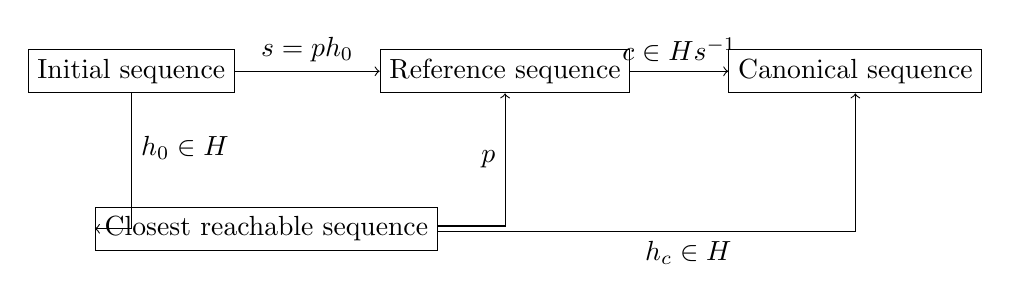
\begin{tikzpicture}
			\node[right, draw] (initial) at (0,0) {Initial sequence};
			\node[draw] (reference) at (0.5\textwidth,0) {Reference sequence};
			\node[left, draw] (canonical) at (\textwidth,0) {Canonical sequence};
			\node[draw] (closest) at (0.25\textwidth,-2) {Closest reachable sequence};

			\draw[->] (initial) -- node[midway, above] {$s = p h_0$} (reference);
			\draw[->] (reference) -- node[midway, above] {$c \in H s^{-1}$} (canonical);
			\draw[->] (initial) |- node[pos=0.2, right] {$h_0 \in H$} (closest);
			\draw[->] (closest.east) ++(0, 0.1em) -| node[pos=0.75, left] {$p$} (reference);
			\draw[->] (closest.east) ++(0, -0.1em) -| node[pos=0.3, below] {$h_c \in H$} (canonical);
		\end{tikzpicture}

		\caption{Illustration of how the canonicalization of a sequence using a canonical coset representative $c$ generated by the determined sort
		permutation $s$ works. Sequence equivalence is determined by the permutations contained in the group $H$.}
		\label{fig:SequenceCanonicalization}
	\end{figure}

	As can be seen in \cref{fig:SequenceCanonicalization}, the permutations that we are interested in would be the $h_0$, that brings the initial
	sequence into an equivalent form that is closest to the reference sequence, and $h_c$ that transforms this closest sequence into the canonical
	sequence. However, these are non-trivial to determine, so we have to take detour. We start by determining the permutation that would transform the
	given sequence into the reference sequence. We call this the sort permutation $s$ as we assume that the reference sequence is simply obtained by
	sorting the elements in our sequence based on some criterion.

	The sort permutation can be thought of as describing a two-step process: first bring the sequence into the closest form and then bring that into
	the reference order. These two steps are formally described by the permutations $h_0$ and $p$ and therefore $s = p h_0$, with
	$h_0 \in H$ by definition.

	We then use the sort permutation to determine the canonical coset representative $c$ of the right coset generated by its inverse and $H$:
	\begin{equation}
		c \in \left( H s^{-1} = \{ h s^{-1} | h \in H \} = \{ h h_0^{-1} p^{-1} | h \in H \} = \{ h_c p^{-1} | h_c \in H \} \right)
	\end{equation}

	Since a group's cosets partition the group, cosets are completely disjoint. That means that there is no permutation that is part of two cosets
	formed by the same subgroup. In our case the group that we are partitioning is simply \Sym{n}, where $n$ is the amount of elements in our sequence
	and the subgroup used to create the cosets is $H$. We want to emphasize that because $H$ contains permutations acting on at most $n$ elements, it
	is necessarily a subgroup of \Sym{n}.

	Since we are inspecting the \emph{right} coset, the $h_0^{-1}$ component in $s^{-1}$ is always multiplied with another permutation $h \in H$,
	which is (by definition) just another element of that same group $H$. Therefore, regardless what $h_0$ originally looked like, we will
	always generate the same coset. Or in other words: Regardless of what of the equivalent index sequences we started with, we will always arrive at
	the same coset (representative).

	Now it is simply a matter of modifying the obtained coset representative in such a way that it can be directly applied to our initial sequence in
	order to transform it into its canonical representation. Since $c$ transforms the reference sequence into the desired canonical representation, we
	can achieve this simply by formally ensuring that our sequence is first transformed into the reference sequence. This is achieved by first acting
	with $s$ on our initial sequence. Therefore, the overall canonicalization permutation is given as
	\begin{equation}
		c s = \underbrace{h_c p^{-1}}_{c} \underbrace{p h_0}_{s} = h_c h_0
	\end{equation}
	which is in perfect agreement with the desired path we want to take in \cref{fig:SequenceCanonicalization} and with our original ansatz for the
	canonicalization.

	Finally, we note that our procedure only relies on being able to determine the sort permutation $p$, which is always possible, and on being able
	to determine the canonnical coset representative. The latter can also be done efficiently when dealing with large groups that are represented
	through a base and a strong generating set as explained by \textcite{Manssur2002a}.


	\appendix

	\section{Dimino's algorithm}
	\label{sec:DiminoAlgorithm}

	An excellent step-by-step derivation of this algorithm can be found in \textcite{Butler1991a}, but we'll sketch the main points here as well.
	Starting point for the Dimino algorithm is a set of generators $S$ that generate a group $G$, which we'll denote $G = \braket{S}$. The algorithm
	then tries to construct all $g \in G$ in an efficient way.

	The fact that $S$ generates $G$, means that every $g \in G$ can be decomposed into a product of generators (note: generators may appear multiple
	times in this decomposition)
	\begin{equation}
		\label{eq:DiminoDecomposition}
		g = \prod_i s_i \hspace{2cm} s_i \in S
	\end{equation}

	Thus, we can perform inductive steps during the generation of $G$.\supercite{Butler1991a} Every element $g$ that requires $m$ generators in
	\cref{eq:DiminoDecomposition} can be expressed as $g = h s$, where $s \in S$ and $h \in G$ is an element that has been generated by multiplying
	$m-1$ generators.\supercite{Butler1991a} This tells us, that when constructing the elements of $g$, it is sufficient to only consider $gs$ as a
	potentially new group element, where $g$ is an element that has already been found to belong to $G$ and $s$ is one of the
	generators.\supercite{Butler1991a}

	Dimino's algorithm ensures that the generators $S = \{ s_0, s_1, \ldots \}$ are processed sequentially. That means that before considering the
	$i$th generator, it first ensures that all possible elements that can be generated by the $s_i$ with $i \in \{0, 1, \ldots, i - 1 \}$ have been
	found and added to $G$.\supercite{Butler1991a} In other words, we first form the complete subgroup that can be generated by the $i-1$ first
	generators, before generating the elements of the group arising from also considering the $i$th generator. The subgroup generated by the first $k$
	generators, will be denoted $H_k$

	The algorithm makes use of the fact that a group is partitioned by the cosets of any of its subgroups.\supercite{Butler1991a} This means that two
	cosets are either completely identical or they have no element in common (they are disjoint). A given coset can simply be generated by forming the
	coset of the subgroup in question with an arbitrary representative of the desired coset\footnote{This is because any specific element can only be
		contained in a single coset. And since a subgroup is itself a \emph{group}, it contains the identity element and therefore the coset formed in
	this way will necessarily contain the element that was used to generate the coset.}. Therefore, if we have generated the subgroup $H_{i-1}$ and
	want to extend it with the generator $s_i$, we simply have to check whether $s_i$ is already contained in $H_{i-1}$. If it is, this generator will
	not yield any new elements and is therefore redundant. If it is not yet contained yet, we can immediately deduce that the entire coset $H_{i-1}
	s_i$ is not yet contained and can therefore add it to $H_i$. If we do add new elements in this way, we'll also have to check whether any of the
	previously processed generators create yet another coset from the coset that has just been added. If they do, we again add the entire coset as new
	elements. This has to be performed in a self-consistent until no new cosets are found. Then we'll have generated the entire subgroup $H_i$ and we
	can move to the next generator $s_{i+1}$ (if any).

	In order to avoid having to compute $\{ h \cdot s_i | \forall h \in H s_n, \forall s_i \in S_i \}$, where $S_i$ is the set of generators processed so
	far and $s_n$ is the just added, new generator, just to find potential new coset representatives, we can instead make use of another coset
	property. If $Hg$ is a coset of $H$ in $G$ and $s_i \in G$ then all elements of $(Hg)s_i$ lie in the coset of $H$ with the coset representative $g
	\cdot s_i$.\supercite{Butler1991a} Or in other words: during our search for new coset representatives, we only have to check the products of the
	old representative with all previously encountered generators, which will save a lot of membership tests.

	From the concepts so far, we can assemble the basic version of Dimino's algorithm by additionally noting that \cref{eq:DiminoDecomposition}
	implies that when only considering a single generator, then the group generated by that is simply given by that generator's
	powers.\supercite{Butler1991a} The result is shown in \cref{alg:DiminoAlgorithm}.

	\begin{algorithm}[!htb]
		\caption{Dimino's algorithm (adapted from \textcite{Butler1991a})}
		\label{alg:DiminoAlgorithm}

		\begin{algorithmic}[1]
			\Function{generateElements}{Set of generators $S$}
				\State \code{elements}: Elements of the to-be-generated group $G$
				\State $s_0 \gets $ first element in $S$
				\ForAll{unique powers of $s_i$ ($s_i^n$)}
				\Comment Generate elements of $G = \braket{s_0}$
					\State Add $s_0^n$ to \code{elements}
				\EndFor
				\For{$i \in [1, $ size of $S) \wedge i \in \mathbb{N}$}
					\Comment{Extend $G$ step-by-step}
					\State $S_{i-1} \gets$ first $i - 1$ entries in $S$
					\State $s_i \gets$ $i$th generator in $S$
					\State \Call{extendGroup}{\code{elements}, $S_{i-1}$, $s_i$}
				\EndFor
			\EndFunction

			\Function{extendGroup}{Elements of group $H$, old generators $S$, new generator $s_n$}
				\If{$s_n \in H$}
				\Comment{New generator is redundant}
					\State \Return
				\EndIf
				\State Add entire coset $H s_n$ to $H$
				\ForAll{cosets added}
					\Comment{Check if any additional cosets to add are found}
					\State $c \gets $ representative of added coset
					\ForAll{$s \in (S \cup \{ s_n \})$}
						\If{$c \cdot s \notin H$}
							\State Add entire coset $H (c \cdot s)$ to $H$
							\Comment This creates another iteration in the outer loop
						\EndIf
					\EndFor
				\EndFor
			\EndFunction
		\end{algorithmic}
	\end{algorithm}

	\textcite{Butler1991a} mentions an additional optimization of this algorithm, that can be applied every time an encountered subgroup happens to be
	\emph{normal}. With this, a few more operations can be saved, but at the expensive of having to implement and run a check whether a given subgroup
	is normal. This optimization has so far not been considered or implemented in \code{libPerm}.

	In the actual implementation of this algorithm it is also possible to leverage the fact, that all cosets of some subgroup $H$ all have the same
	size: $|H|$.


	\section{Defining ordering between permutations}
	\label{sec:OrderPermutations}

	The process for introducing a total ordering of permutations is taken from \textcite{Manssur2002a}. It starts by introducing a list $\mathbf{b} =
	[b_0, b_1, \ldots]$ of $N$ distinct numbers of the set $\{ 0, 1, \ldots, n = N - 1 \}$, where $n$ is the biggest point that is permuted by any of
	the permutations that are supposed to be compared.

	This list of points allows us to define the order of points. $\alpha \prec \beta$, if $\alpha$ comes before $\beta$ in $\mathbf{b}$
	(left-to-right).\supercite{Manssur2002a}

	We define $\mathbf{b}^p = [ b_0^p, b_1^p, \ldots ]$ as the image of $\mathbf{b}$ under the permutation $p$. Such lists of points are compared
	element-wise, such that $\mathbf{b}^p \prec \mathbf{b}^q$ if for the first (left-to-right) point $\alpha \in \mathbf{b}^p, \beta \in \mathbf{b}^q$
	for which $\alpha \neq \beta$, it is $\alpha \prec \beta$.\supercite{Manssur2002a}

	The relative order between permutations is then simply based on the order of the images of $\mathbf{b}$ under the permutations. For two
	permutations $p,q$, we therefore define\supercite{Manssur2002a}
	\begin{equation}
		p \prec q \iff \mathbf{b}^p \prec \mathbf{b}^q
	\end{equation}

	Inside \code{PermLib}, our permutations also carry sign information, but since the same permutation can't be contained in a single group with both
	possible sign values\supercite{Manssur2002a}, we can simply ignore the sign when comparing permutations.\supercite{Manssur2002a}

	We want to put emphasize on the fact that the choice of a specific $\mathbf{b}$ to use for defining order is arbitrary. Certain situations might
	make it beneficial to select the points and their order in $\mathbf{b}$ in a specific way, but this has no effect on the concepts used to define
	ordering. It may, however, affect the specific order established this way. Therefore, it is important to consistently use the same $\mathbf{b}$
	throughout a given (part of a) code.


	\cleardoublepage
	\printbibliography

\end{document}
